% Originally: content/week-03.tex, \section{Path connectedness} (Corsin Week 3, Friday)

\section{Path connectedness}
\label{sec:path_connectedness}

% Transition: Claude Opus 5 (High)
\Cref{def:connectedness} defines connectedness negatively. A space is connected when it
\emph{cannot} be split, which is why proofs about it run by contradiction. That is mathematically
convenient and intuitively unsatisfying, since it says nothing whatever about what holds a
connected space together.

Path connectedness is the positive version, and it says the obvious thing: any two points can be
joined by a curve running inside the space. It implies connectedness
(\cref{lem:path_connected_implies_connected}), and on open subsets of $\mathbb{R}^n$ the two
notions agree (\cref{prop:open_euclidean_connected_path_connected}). In general they come apart,
and the topologist's sine curve at the end of this section is the standard witness.

% Source: Corsin Nick/Class Notes/Week 3.pdf, pp. 1--14
\begin{definition}[Path]
\label{def:path}
Let $(X,d)$ be a metric space. A continuous function $\gamma : [0,1] \to X$, where $[0,1]$
carries the standard metric, is called a \newterm{path} (\germanterm{Weg}). More generally, we
can replace $[0,1]$ by $[a,b]$ for $a < b$.
\end{definition}

\begin{definition}[Path-connected]
\label{def:path_connected}
A metric space $X$ (or subset thereof) is \newterm{path-connected}
(\germanterm{wegzusammenh\"angend}) if for all $x, y \in X$ there exists a path
(\cref{def:path}) $\gamma : [0,1] \to X$ with $\gamma(0) = x$, $\gamma(1) = y$.
\begin{center}
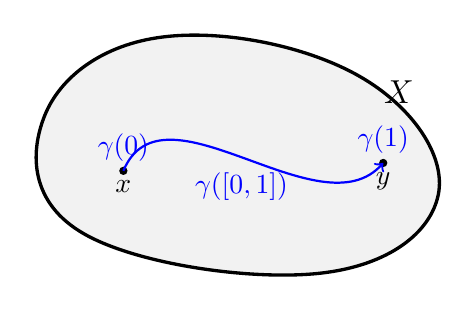
\begin{tikzpicture}
  \draw[very thick, fill=gray!10] plot[smooth cycle, tension=0.7] coordinates {(-2, -1) (-2.5, 0.5) (-1, 1.5) (1.5, 1) (2.5, -0.5) (1, -1.5)};
  \node[font=\large] at (2, 0.8) {$X$};
  
  \fill (-1.5, -0.2) circle (1.5pt) node[below] {$x$};
  \fill (1.8, -0.1) circle (1.5pt) node[below] {$y$};
  
  \draw[blue, thick, ->] (-1.5, -0.2) .. controls (-1, 1) and (1, -1) .. (1.8, -0.1);
  
  \node[blue, above] at (-1.5, -0.2) {$\gamma(0)$};
  \node[blue, above] at (1.8, -0.1) {$\gamma(1)$};
  \node[blue, below] at (0, -0.1) {$\gamma([0,1])$};
\end{tikzpicture}
\end{center}
\end{definition}

\begin{lemma}[Path-connected implies connected]
\label{lem:path_connected_implies_connected}
Let $X$ be a metric space. Then $X$ path-connected (\cref{def:path_connected}) implies $X$
connected (\cref{def:connectedness}).
\end{lemma}

% Generator: Claude Opus 5 (High) --- stated without proof in the source.
\begin{proof}
Suppose $X$ were path-connected but disconnected, say $X = U_1 \sqcup U_2$ with $U_1,U_2$ open,
disjoint and non-empty. Pick $x \in U_1$, $y \in U_2$ and a path $\gamma : [0,1] \to X$ with
$\gamma(0)=x$, $\gamma(1)=y$. Then $\gamma^{-1}(U_1)$ and $\gamma^{-1}(U_2)$ are open in $[0,1]$
by \cref{def:continuous}\textbf{(c)}, disjoint, cover $[0,1]$, and are non-empty (they contain
$0$ and $1$ respectively). This disconnects $[0,1]$, contradicting
\cref{prop:intervals_connected}.
\end{proof}

% Source: Jérôme Paschoud/Notizen/Woche 3.1 Banach und Kompaktheit.pdf, p. 6
% Generator: Gemini 3.6 Flash (High)
\begin{exercise}[The unit disk is connected]
\label{ex:disk_connected}
Prove that the set $S^1 := \{ (x,y) \in \mathbb{R}^2 \mid x^2 + y^2 \leq 1 \}$ is connected.
\end{exercise}

\begin{exercisesolution}[Proof of \cref{ex:disk_connected}]
Instead of proving connectedness directly via open sets, we can show that $S^1$ is path-connected, which implies connectedness (\cref{lem:path_connected_implies_connected}). Given any two points $a, b \in S^1$, we can connect them via a straight line segment. The segment can be parameterized as $\gamma(t) := (1-t)a + tb$ for $t \in [0,1]$. Since $S^1$ (the unit disk in $\mathbb{R}^2$) is convex, for any $t \in [0,1]$ we have $\lVert \gamma(t) \rVert \leq (1-t)\lVert a \rVert + t \lVert b \rVert \leq 1-t + t = 1$, so the entire path lies in $S^1$. Because any two points can be connected by a continuous path within $S^1$, the set is path-connected, and therefore connected.

(Note: The standard notation for the unit disk is $D^2$ or $B_1(0)$, whereas $S^1$ usually denotes the boundary circle $\{x^2+y^2=1\}$, but we reproduce the notation $S^1$ here as it appears in the source notes.)
\end{exercisesolution}

\begin{proposition}[Connectedness and path-connectedness in open Euclidean subsets]
\label{prop:open_euclidean_connected_path_connected}
Let $U \subseteq \mathbb{R}^n$ be open (\cref{def:open_closed}). Then
\[
U \text{ path-connected} \iff U \text{ connected}.
\]
\end{proposition}

% Generator: Claude Opus 5 (High) --- stated without proof in the source; the "(<=)" direction
% is the standard "the set of reachable points is clopen" argument and is worth having, since it
% is the only place in this chapter where openness is genuinely used.
\begin{proof}
\textbf{($\Rightarrow$)} is \cref{lem:path_connected_implies_connected}, which needs neither
openness nor $\mathbb{R}^n$.

\textbf{($\Leftarrow$)} Assume $U$ is connected and non-empty (the empty set is vacuously
path-connected), and fix $x_0 \in U$. Let
\[A := \{x \in U \ :\ \text{some path in } U \text{ joins } x_0 \text{ to } x\}.\]
We show $A$ and $U \setminus A$ are both open; since $x_0 \in A$ (take the constant path),
connectedness then forces $U\setminus A = \emptyset$, i.e.\ $A = U$, which is the claim.

Let $x \in U$ and choose $r>0$ with $B_r(x) \subseteq U$, using that $U$ is open. The ball is
convex, so every $y \in B_r(x)$ is joined to $x$ by the straight segment
$t \mapsto (1-t)x+ty$, which stays inside $B_r(x) \subseteq U$. Consequently:
\begin{itemize}
  \item If $x \in A$, concatenating a path from $x_0$ to $x$ with that segment joins $x_0$ to
    any $y \in B_r(x)$, so $B_r(x) \subseteq A$ and $A$ is open.
  \item If $x \notin A$, then no $y \in B_r(x)$ can lie in $A$, since otherwise running the
    segment backwards from $y$ to $x$ would join $x_0$ to $x$. So $B_r(x) \subseteq U\setminus A$ and
    $U\setminus A$ is open.
\end{itemize}
(Concatenation of two paths is again a path: traverse the first on $[0,\tfrac12]$ and the second
on $[\tfrac12,1]$, each at double speed; the result is continuous because the two pieces agree
at $t=\tfrac12$.)
\end{proof}

\begin{importantremark}[Only for open subsets]
\label{rem:path_connected_needs_open}
The implication \qt{connected $\Rightarrow$ path-connected} is \emph{false} without openness,
and the proof shows exactly why: the ball $B_r(x)$ around a point of $U$ was needed to supply
the straight segment. For a set that is not open there may be points with no room around them at
all, and the topologist's sine curve (\cref{ex:topologists_sine_curve}) below is precisely such
a case. There the origin has no neighbourhood in $S$ that is a nice piece of curve.
\end{importantremark}

% Source: Corsin Nick/Class Notes/Week 3.pdf, pp. 1--14
% (Re-cited: the two proofs and the important remark above are additions, not transcription.)
\begin{example}[The topologist's sine curve]
\label{ex:topologists_sine_curve}
\[S := \left\{\left(t, \sin\left(\tfrac{1}{t}\right)\right) : t > 0\right\} \cup \{(0,0)\} \subseteq \mathbb{R}^2\]
$S$ is \textbf{connected} but \textbf{not path-connected}!
\end{example}

\begin{ainote}
Corsin writes the second piece as $\cup\,\{0\}$; since $S \subseteq \mathbb{R}^2$, the point
being adjoined is the origin $(0,0) \in \mathbb{R}^2$, not the number $0$. Written as
$\cup\,\{(0,0)\}$ above, which is also what his own figure and the proof below use.
\end{ainote}

\begin{center}
\begin{tikzpicture}[>=Latex, scale=1.3]
  \draw[->] (-0.2,0) -- (3.2,0) node[right] {$t$};
  \draw[->] (0,-1.4) -- (0,1.4) node[above] {$y$};
  \draw (0,1.0) -- (-0.05,1.0) node[left, font=\footnotesize] {$1$};
  \draw (0,-1.0) -- (-0.05,-1.0) node[left, font=\footnotesize] {$-1$};
  % Horizontal figure-coordinate \x corresponds to t = \x/10, since the plot is sin(10/\x).
  \draw (1.0,0.05) -- (1.0,-0.05) node[below, font=\footnotesize] {$0.1$};
  \draw (2.0,0.05) -- (2.0,-0.05) node[below, font=\footnotesize] {$0.2$};

  \draw[blue!80!black, thick] plot[domain=0.08:2.8, samples=250] (\x, {sin((1.0/(\x*0.1)) r)});
  \fill[blue!80!black] (0,0) circle (1.5pt) node[left, font=\footnotesize] {$(0,0)$};
  \node[above, font=\small] at (1.5,1.3) {$S = \{(t, {\sin(1/t})) : t > 0\} \cup \{(0,0)\}$};
\end{tikzpicture}
\end{center}

\begin{proof}[$S$ is connected]
Write $G := S \setminus \{(0,0)\} = \{(t,\sin(1/t)) : t>0\}$ for the graph part, and suppose for
contradiction that $S$ is disconnected, say $S = V_1 \sqcup V_2$ with $V_1,V_2$ non-empty,
disjoint and open in $S$. Say $(0,0) \in V_1$.

$G$ is the continuous image of the interval $(0,\infty)$ under
$t \mapsto (t,\sin(1/t))$, hence path-connected, hence connected
(\cref{lem:path_connected_implies_connected}). A connected set meeting both parts of a
separation would itself be separated, so $G$ lies entirely in $V_1$ or entirely in $V_2$.

It cannot lie in $V_1$: then $V_2 \subseteq S \setminus (G \cup \{(0,0)\}) = \emptyset$,
contradicting $V_2 \neq \emptyset$. So $G \subseteq V_2$, and therefore
$V_1 = \{(0,0)\}$.

But $V_1$ is open in $S$, so some ball $B_\varepsilon\big((0,0)\big) \cap S$ equals
$\{(0,0)\}$, and that is false. For $t := \tfrac{1}{k\pi}$ with $k$ large, the point
$(t,\sin(1/t)) = (t,0) \in G$ lies within $\varepsilon$ of the origin. This is the required
contradiction, so $S$ is connected.
\end{proof}

\begin{proof}[$S$ is not path-connected]
Assume by contradiction there is a path from $(0,0)$ to $(\tfrac{1}{\pi}, 0)$,
\[
\gamma : [0,1] \to [0, \tfrac{1}{\pi}] \times [-1,1], \qquad t \mapsto (x(t), y(t)).
\]
Since $\gamma$ is continuous, $x$ and $y$ must also be continuous. By the \newterm{intermediate
value theorem} (\cref{cor:intermediate_value_theorem}), $x : [0,1] \to [0,\tfrac{1}{\pi}]$
attains every value in $[0,\tfrac{1}{\pi}]$, since $x(0) = 0$ and $x(1) = \tfrac{1}{\pi}$.
Therefore, we find a sequence $(a_n)_{n=1}^{\infty}$ such that
\[
x(a_n) = \frac{1}{2\pi n + \tfrac{\pi}{2}}.
\]
We may moreover choose the $a_n$ \textbf{decreasing}: having found $a_{n-1}$, apply the
intermediate value theorem on $[0,a_{n-1}]$ rather than on $[0,1]$, which is legitimate because
$x(0) = 0$ and $x(a_{n-1}) = \tfrac{1}{2\pi(n-1)+\pi/2}$ already straddle the next target value.
This yields $a_n \in (0,a_{n-1})$, so $(a_n)$ is decreasing and bounded below, hence convergent,
say $a_n \to \ell \in [0,1]$.

Now evaluate $\gamma$ along this sequence. By construction $x(a_n) \to 0$, so continuity gives
$x(\ell) = 0$; and $y(a_n) = \sin\!\big(2\pi n + \tfrac\pi2\big) = 1$ for every $n$, so
$y(\ell) = 1$. Hence $\gamma(\ell) = (0,1)$. But $(0,1) \notin S$: the only point of $S$ whose
first coordinate vanishes is the origin. This contradicts $\gamma([0,1]) \subseteq S$, so no
such path exists.
\end{proof}

\begin{ainote}
Corsin's argument produces the $a_n$ from the intermediate value theorem and then asserts
$a_n \to 0$. That does not follow from the choice as stated. The intermediate value theorem
returns \emph{some} preimage, and nothing so far prevents all of them from sitting near $1$.
The repair is the standard one and costs one sentence: apply the theorem on the shrinking
intervals $[0,a_{n-1}]$ rather than on $[0,1]$ each time, which forces the $a_n$ down. Inserted
above; the rest of his proof is unchanged.
\end{ainote}

\begin{center}
\begin{tikzpicture}[>=Latex, scale=1.3]
  \draw[->] (-0.3,0) -- (3.2,0) node[right] {$t$};
  \draw[->] (0,-1.4) -- (0,1.4) node[above] {$y$};

  \draw[blue!80!black, thick] plot[domain=0.08:2.8, samples=250] (\x, {sin((1.0/(\x*0.1)) r)});

  \fill[red!80!black] (0,0) circle (2pt) node[below left, font=\small] {$\gamma(0)$};

  % The peaks of the plotted sin(10/x) sit at x = 20/(pi(1+4k)), k = 1,2,3,...
  % -- these must land ON the curve, since they are the points gamma(a_n).
  \fill[red!80!black] (1.273,1.0) circle (2pt) node[above right, font=\footnotesize] {$\gamma(a_1)$};
  \fill[red!80!black] (0.707,1.0) circle (1.7pt);
  \fill[red!80!black] (0.490,1.0) circle (1.4pt);
  \fill[red!80!black] (0.374,1.0) circle (1.1pt);
  \fill[red!80!black] (0.303,1.0) circle (0.9pt);

  % The limit (0,1) is NOT a point of S -- hence the hollow circle.
  \draw[red!80!black, thick] (0,1.0) circle (2.5pt);
  \node[red!80!black, font=\footnotesize, left] at (-0.08,1.0) {$(0,1)$};
  \draw[red!80!black, ->, dashed] (1.15,1.19) -- (0.13,1.07);

  \node[red!80!black, font=\small] at (1.75,-1.15) {$\gamma(a_n) \to (0,1) \neq (0,0) = \gamma(0)$};
\end{tikzpicture}
\end{center}

% Sonnet 5 (Medium)
We close the week with a change of subject: away from topology and back to the linear-algebraic
structure (\cref{sec:structured_spaces}) that lets us talk about angles, not just distances.



% Originally: content/week-03.tex, end of \subsection{Contraction mappings}

\begin{aiexercise}[Continuous image of a path-connected set]
\label{ex:ai_connected_image}
% Generator: Claude Opus 5 (High). Replaces an earlier exercise asking for
% \cref{thm:continuity_preserves_connected}, which now carries its own proof.
Let $f \colon X \to Y$ be a continuous map between metric spaces.
\begin{enumerate}[label=\textbf{(\alph*)}]
  \item Prove that if $X$ is path-connected (\cref{def:path_connected}), then so is $f(X)$.
  \item Conclude that the graph $\Gamma_g := \{(x,g(x)) : x \in U\}$ of a continuous
    $g : U \to \mathbb{R}^m$ is path-connected whenever $U \subseteq \mathbb{R}^n$ is convex.
    (Compare \cref{ex:4.2}, which asks the same question with \qt{connected} in place
    of \qt{path-connected}.)
\end{enumerate}
\end{aiexercise}

% --- exercise relocated here from the dissolved sheet 4 ---

% Originally: content/week-04.tex, \exercisesheet{4}
% Source: exercises/Ex4_Analysis2_eng.pdf

\begin{exercise}[4.2 --- Connected graphs \textnormal{(important)}]
\label{ex:4.2}
Let $U \subset \mathbb{R}^n$ be open and connected and let $f \in C^1(U, \mathbb{R}^m)$. Show that
its graph
\[\Gamma_f := \{(x, f(x)) : x \in U\}\]
is a connected subset of $\mathbb{R}^n \times \mathbb{R}^m$.
\end{exercise}
